\begin{subsectionframemod}{Difference between Natural and Aerial Images}
    \metroset{block=fill}
    \begin{alertblock}{LoRA (Low-Rank Adaptation)}
        LoRA (Low-Rank Adaptation) est une technique d'optimisation qui ajuste efficacement les modèles de réseaux neuronaux de grande taille en réduisant le nombre de paramètres à ajuster via la factorisation des matrices de poids.
        En limitant le nombre de paramètres modifiés, elle aide également à réduire le risque d'overfitting tout en maintenant de bonnes performances.
    \end{alertblock}
    \vspace{5mm}

    \begin{figure}
        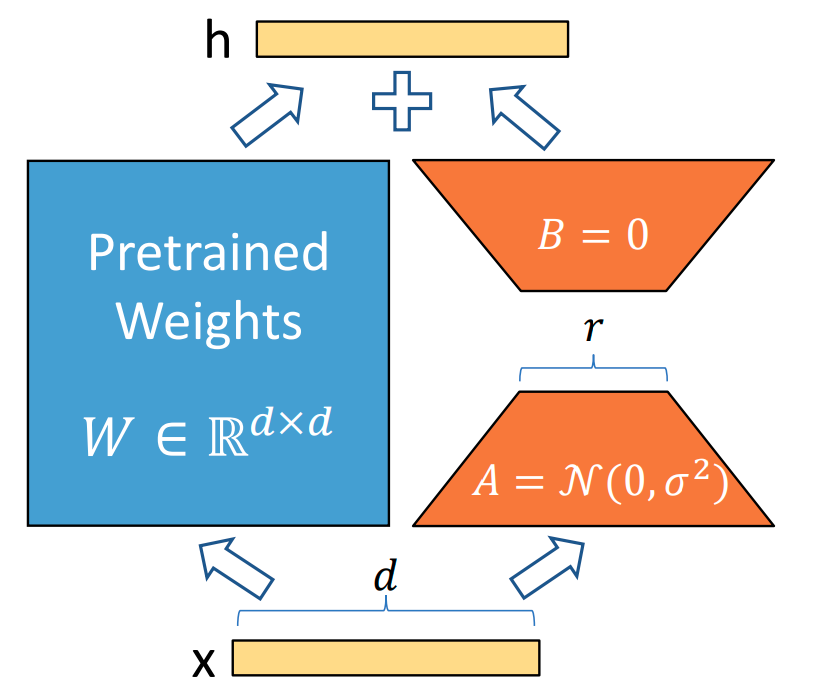
\includegraphics[width=0.4\textwidth]{Figures/lora.png}
        \caption{Principe de l'entrainement LoRA. Ici on entraine seulement A et B (\cite{lora}).}
    \end{figure}


\end{subsectionframemod}